\documentclass[12pt,a4paper]{article}

\usepackage[utf8]{inputenc}
\usepackage[T1]{fontenc}
\usepackage{tgtermes}
\usepackage[scaled=0.92]{helvet}
\usepackage[a4paper,
    left=56.7pt,
    right=53.6pt,
    top=108pt,
    bottom=66pt
]{geometry}
\usepackage{amsmath,amssymb,amsfonts}
\usepackage{booktabs,multirow,tabularx}
\usepackage{graphicx}
\usepackage{xcolor}
\usepackage{tikz}
\usetikzlibrary{shapes.geometric,arrows.meta,positioning,calc,fit,backgrounds}
\usepackage{pgfplots}
\pgfplotsset{compat=1.18}
\usepackage{hyperref}
\usepackage{microtype}
\usepackage{enumitem}
\usepackage{titlesec}
\usepackage{eso-pic}
\usepackage{setspace}
\usepackage{algorithm}
\usepackage{algorithmic}
\usepackage{caption}

\definecolor{journalnavy}{RGB}{0,31,95}
\definecolor{linkdoi}{RGB}{0,0,222}
\definecolor{linkblue}{RGB}{79,129,189}

\pagestyle{empty}

% Exact Page Border & Perfectly Centered Header / Footer
\AddToShipoutPictureBG{%
  \begin{tikzpicture}[remember picture, overlay]
    % Border (24pt box matching IJARCCE)
    \draw[black, line width=0.5pt]
      ([shift={(24.0pt,-24.0pt)}]current page.north west)
      rectangle
      ([shift={(-24.0pt,24.0pt)}]current page.south east);

    % Header - Exactly Centered IJARCCE
    \node[anchor=center] at ([yshift=-45.5pt]current page.north) {%
      {\fontfamily{phv}\selectfont\textbf{\fontsize{16pt}{18pt}\selectfont IJARCCE}}%
    };
    \node[anchor=east] at ([shift={(-53.6pt,-46.5pt)}]current page.north east) {%
      {\fontfamily{phv}\selectfont\fontsize{8pt}{10pt}\selectfont ISSN (O) 2278-1021, ISSN (P) 2319-5940}%
    };
    \node[anchor=west] at ([shift={(56.7pt,-69.1pt)}]current page.north west) {%
      
\includegraphics[width=20.7pt,height=16.8pt]{ijarcce_logo.png}%
    };
    \node[anchor=center] at ([yshift=-69.1pt]current page.north) {%
      {\color{journalnavy}\fontfamily{phv}\selectfont\textbf{\fontsize{9.5pt}{11pt}\selectfont International Journal of Advanced Research in Computer and Communication Engineering}}%
    };
    \node[anchor=center] at ([yshift=-84.8pt]current page.north) {%
      {\fontfamily{phv}\selectfont\textbf{\fontsize{8.5pt}{10pt}\selectfont Impact Factor 8.102 \quad $\bowtie$ \quad Peer-reviewed / Refereed journal \quad $\bowtie$ \quad Vol. 15, Issue x, Month 2026}}%
    };
    \node[anchor=center] at ([yshift=-99.8pt]current page.north) {%
      {\color{linkdoi}\fontfamily{phv}\selectfont\textbf{\fontsize{9pt}{11pt}\selectfont DOI: 10.17148/IJARCCE.2026.14xx}}%
    };

    % Footer
    \node[anchor=west] at ([shift={(56.7pt, 41.5pt)}]current page.south west) {%
      {\fontsize{10pt}{12pt}\selectfont\textbf{\copyright}\hspace{3pt}{\color{blue}\textbf{IJARCCE}}}%
    };
    \node[anchor=center] at ([yshift=41.5pt]current page.south) {%
      {\fontsize{9pt}{11pt}\selectfont\textbf{This work is licensed under a Creative Commons Attribution 4.0 International License}}%
    };
    \node[anchor=east] at ([shift={(-53.6pt, 41.5pt)}]current page.south east) {%
      {\fontsize{9pt}{11pt}\selectfont\textbf{\thepage}}%
    };
  \end{tikzpicture}%
}

% Paragraph formatting
\setlength{\parindent}{0pt}
\setlength{\parskip}{3.0pt}
\linespread{1.04}

% Float and caption spacing
\setlength{\floatsep}{5pt plus 2pt minus 1pt}
\setlength{\textfloatsep}{7pt plus 2pt minus 2pt}
\setlength{\intextsep}{5pt plus 2pt minus 1pt}
\setlength{\abovecaptionskip}{3pt}
\setlength{\belowcaptionskip}{2pt}

% Section formatting matching IJARCCE reference paper (12pt Bold Times New Roman)
\titleformat{\section}{\fontsize{12pt}{14pt}\selectfont\bfseries}{\thesection.}{0.5em}{}
\titleformat{\subsection}{\fontsize{12pt}{14pt}\selectfont\bfseries}{\thesubsection}{0.5em}{}
\titleformat{\subsubsection}{\fontsize{12pt}{14pt}\selectfont\bfseries}{\thesubsubsection}{0.5em}{}
\titlespacing*{\section}{0pt}{6pt plus 1pt minus 1pt}{2pt plus 0.5pt}
\titlespacing*{\subsection}{0pt}{5pt plus 1pt minus 0.5pt}{1.5pt plus 0.5pt}
\titlespacing*{\subsubsection}{0pt}{5pt plus 1pt minus 0.5pt}{2pt}

% Captions formatting
\captionsetup[figure]{name=Figure,labelsep=period,font={small,bf},justification=centering,skip=3pt}
\captionsetup[table]{name=Table,labelsep=period,font={small,bf},justification=centering,skip=3pt}

\hypersetup{
    colorlinks=true,
    linkcolor=black,
    citecolor=black,
    urlcolor=linkblue
}


\renewcommand{\topfraction}{0.88}
\renewcommand{\bottomfraction}{0.88}
\renewcommand{\textfraction}{0.08}
\renewcommand{\floatpagefraction}{0.88}

\begin{document}

% Title Block
\begin{center}
  {\fontfamily{phv}\selectfont\textbf{\fontsize{16pt}{20pt}\selectfont Real-Time Coding Contests in College Programming Labs:\\[3pt] A Case Study at RCPIT Shirpur}}\par
  \vspace{8pt}
  {\fontsize{12pt}{15pt}\selectfont\textbf{Sachin Narendra Chaudhari$^{1}$, Jayesh Rameshsing Girase$^{2}$, Sakshi Dadabhau Patil$^{3}$,\\[2pt] Chetan Prabhakar Sonawane$^{4}$, Dr. N. G. Shinde$^{5}$}}\par
  \vspace{7pt}
  {\fontsize{10pt}{13pt}\selectfont
  $^{1}$ UG student, SES's R. C. Patel Institute of Technology, Shirpur 425405 India,
  {\color{linkblue}\underline{\textbf{sachinchau1055@gmail.com}}}\par
  \vspace{2pt}
  $^{2}$ UG student, SES's R. C. Patel Institute of Technology, Shirpur 425405 India,
  {\color{linkblue}\underline{\textbf{jayeshgirase29@gmail.com}}}\par
  \vspace{2pt}
  $^{3}$ UG student, SES's R. C. Patel Institute of Technology, Shirpur 425405 India,
  {\color{linkblue}\underline{\textbf{sakshi.p3637@gmail.com}}}\par
  \vspace{2pt}
  $^{4}$ UG student, SES's R. C. Patel Institute of Technology, Shirpur 425405 India,
  {\color{linkblue}\underline{\textbf{chetansonawane1783@gmail.com}}}\par
  \vspace{2pt}
  $^{5}$ Associate Professor, Department of Artificial Intelligence and Machine Learning,\\[1pt]
  SES's R. C. Patel Institute of Technology, Shirpur 425405 India,
  {\color{linkblue}\underline{\textbf{nitin.shinde@rcpit.ac.in}}}\par
  }\par
\end{center}

\vspace{3pt}

\textbf{\fontsize{12pt}{14pt}\selectfont Abstract}

Data Structures and Algorithms (DSA) is a core subject in undergraduate computer engineering and artificial intelligence curricula. In most engineering colleges, programming practicals follow an open-ended lab format where students work at their own pace and submit unfinished tasks as homework. Under this model, instructors frequently observe three challenges: students postpone coding until the weekend deadline, make repeated trial-and-error submissions instead of thinking through logic, and struggle on proctored practical exams. To address these problems, we created and deployed \textbf{Campus Lab}, an open-source web platform for college computer laboratories. Campus Lab brings real-time, timed contest rooms and sandboxed code execution (using Judge0 CE) directly to the departmental local area network (LAN). Instructors run 90-minute contests during standard two-hour practical sessions, offering instant feedback on sample tests and a live room leaderboard. We evaluated Campus Lab in a 16-week crossover study with 64 sophomore Artificial Intelligence and Machine Learning students at R. C. Patel Institute of Technology (RCPIT), Shirpur, split into two batches ($n = 32$ each). Students in contest mode completed $88.5\%$ of assigned problems during lab hours, compared to $61.2\%$ in traditional homework mode. On proctored practical exams, students scored $5.8$ marks higher (out of 50) on topics learned through contest rooms. Formal submissions per solved problem dropped from $5.7$ to $3.2$, as students made use of sample test runs and planned their logic before submitting. Survey responses showed strong student enthusiasm for contest-driven labs when grading prioritized problem completion rather than leaderboard speed. We share four practical recommendations for engineering colleges adopting in-class contest platforms.

\vspace{4pt}

% =========================================================================
\section{Introduction}
\label{sec:intro}
% =========================================================================

\subsection{Practical Challenges in College Programming Labs}
Data Structures and Algorithms (DSA) is essential for computer science and artificial intelligence students [1]. Mastering DSA requires understanding algorithmic complexity and developing solid hands-on coding and debugging skills [2]. In Indian engineering institutions, including R. C. Patel Institute of Technology (RCPIT), Shirpur, undergraduate students in Artificial Intelligence and Machine Learning (AI\&ML) complete DSA practicals in their sophomore year (Second Year, B.Tech). The curriculum combines weekly theory lectures with scheduled two-hour laboratory sessions in departmental computer centers.

Despite its importance, the conventional format of college programming labs faces three recurring hurdles:
\begin{enumerate}[leftmargin=1.5em, itemsep=1pt]
    \item \textbf{Procrastination on Take-Home Assignments:} In typical two-hour lab periods, students often work slowly or get delayed by minor syntax errors. Incomplete tasks turn into take-home homework due Sunday night. More than $60\%$ of submissions arrive in the final hours before the cutoff, resulting in rushed code and superficial learning [5].
    \item \textbf{Guess-and-Check Debugging Habits:} Working at home without immediate faculty guidance, students often make small trial edits and repeatedly submit to guess hidden test cases [6]. This trial-and-error habit prevents them from systematically tracing code logic on paper.
    \item \textbf{Low Engagement During Lab Slots:} Without an immediate, structured target within the two-hour lab session, laboratory hours become passive. Students miss out on focused peer discussion and real-time instructor feedback.
\end{enumerate}

\subsection{Motivation for In-House Contest Rooms}
Automated Assessment Systems (AAS) evaluate student programming code automatically [3, 4]. Commercial platforms such as LeetCode, HackerRank, and Codeforces have shown that timed contests and live leaderboards create strong motivation [7]. However, public platforms are designed for individual online practice rather than supervised college laboratories. They rely entirely on external internet connections, cannot authenticate students with institutional Permanent Registration Numbers (PRNs), and feature problem sets that do not align with university course curricula [9].

To solve these challenges, we built \textbf{Campus Lab}. Deployed directly on an on-premise departmental server over the college local area network (LAN), Campus Lab offers real-time contest rooms, an isolated Judge0 code runner supporting C++, Java, and Python, and curated problems aligned with the academic syllabus.

\subsection{Research Questions}
We deployed Campus Lab at RCPIT Shirpur across a full 16-week semester to examine four research questions:
\begin{itemize}[leftmargin=1.5em, itemsep=1pt]
    \item \textbf{RQ1 (Exam Performance):} Does practicing DSA problems in timed contest rooms improve scores on individual, proctored practical exams compared to take-home homework?
    \item \textbf{RQ2 (Debugging Habits):} How does the synchronous contest format affect student submission attempts, sample test runs, and compilation errors?
    \item \textbf{RQ3 (Lab Completion):} Does real-time contest participation increase the proportion of problems completed during scheduled lab hours and decrease deadline rushes?
    \item \textbf{RQ4 (Student Perceptions):} How do students, including beginners and female students, perceive in-class contests, and does the format cause undue anxiety?
\end{itemize}

% =========================================================================
\section{Related Work}
\label{sec:related}
% =========================================================================

\subsection{Automated Assessment in Programming Education}
Automated grading tools have gained wide adoption in computer science education [3, 10]. Systems like Web-CAT [11] and Marmoset [5] showed that instant automated feedback motivates students to start coding earlier. Nevertheless, researchers caution that automated grading alone does not create sound debugging habits [4, 12]. When students receive fail messages without teacher input, they often enter repetitive submission loops [6]. Automated grading is most beneficial when paired with structured lab pacing and in-person instructor guidance.

\subsection{Gamification and In-Class Coding Contests}
Gamification techniques, such as points and live leaderboards, draw on students' intrinsic motivation and peer camaraderie [8, 13]. Research in computing education indicates that contest formats raise student interest and time on task [14]. However, public leaderboards can induce stress, particularly for beginners and underrepresented groups, if rankings affect grades [15]. A successful classroom contest environment must therefore keep leaderboard dynamics friendly and low-stakes, ensuring that marks reward problem completion rather than speed [16].

\subsection{Synchronous Lab Practice vs. Take-Home Homework}
Practicing programming synchronously in physical labs provides clear advantages over remote homework [17]. When writing code alongside peers and instructors, students receive immediate assistance when encountering conceptual blockers. This minimizes frustration and keeps students moving forward. However, standard practical sessions often suffer from low output because students lack concrete in-lab targets. Timed contest rooms provide this structure by setting clear, achievable milestones during the laboratory period.

Table~\ref{tab:comparison} compares existing programming tools with Campus Lab across institutional requirements.

\begin{table}[!htbp]
\centering
\small
\caption{Comparison of Existing Programming Platforms with Campus Lab}
\label{tab:comparison}
\begin{tabularx}{\linewidth}{|l|l|X|X|}
\hline
\textbf{Platform} & \textbf{Deployment} & \textbf{Key Advantages} & \textbf{Key Limitations in College Labs} \\
\hline
LeetCode / Codeforces & Public Cloud & Large problem library, active global community & Requires internet; no college PRN integration; problems misaligned with syllabus \\
\hline
HackerRank for Education & Cloud SaaS & Good assessment tools, pre-built coding tests & Recurring license cost; external dependency; limited custom contest customization \\
\hline
Web-CAT / Marmoset & Campus Server & Automated unit test grading, student effort tracking & Lacks live synchronous contest rooms; outdated user interfaces; no live leaderboard \\
\hline
\textbf{Campus Lab (Proposed)} & \textbf{Local LAN Server} & \textbf{Zero internet dependency; live contest rooms; institutional PRN auth; dual-stage runs} & \textbf{Requires initial local server setup and departmental administration} \\
\hline
\end{tabularx}
\end{table}

% =========================================================================
\section{The Campus Lab Platform}
\label{sec:platform}
% =========================================================================

\subsection{Platform Architecture and Departmental Deployment}
Campus Lab is designed as a self-contained four-tier web application running entirely on an institutional server on the college local area network (LAN):
\begin{itemize}[leftmargin=1.5em, itemsep=1.5pt]
    \item \textbf{Client Tier:} A responsive single-page web app built with React 19 and Vite. The editor uses CodeMirror 6 with full syntax highlighting, bracket matching, and auto-indentation for C++, Java, and Python. The interface features split panels for problem descriptions, sample inputs/outputs, terminal outputs, and live room leaderboards.
    \item \textbf{API Server:} A modular backend built with Node.js and Express 5 in TypeScript. It handles student authentication using institutional Permanent Registration Numbers (PRNs), contest room timers, and submission dispatching.
    \item \textbf{Database Tier:} A PostgreSQL 16 database managed through Prisma 7 ORM. It stores curated problems, test cases, room standings, and student submission histories.
    \item \textbf{Code Execution Sandbox:} An isolated Judge0 CE instance running in Docker containers. Student code is executed under strict Linux cgroup limits: a 2.0-second CPU execution cap and a 256MB RAM cap, preventing runaway processes or infinite loops from affecting system stability [9].
\end{itemize}

Figure~\ref{fig:architecture} illustrates the system architecture and data flow between client workstations, the API server, the database, and the execution sandbox.

\begin{figure}[!htbp]
\centering
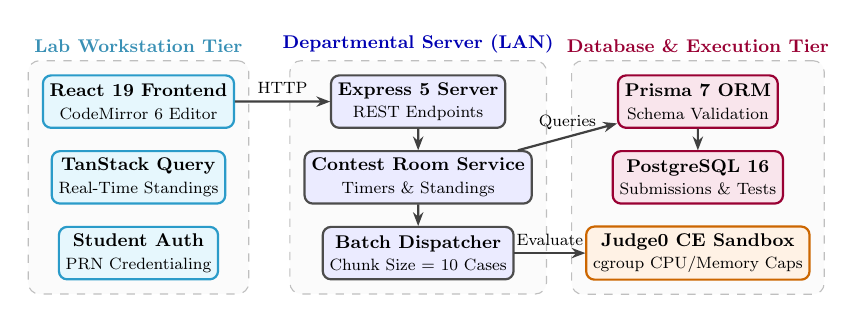
\begin{tikzpicture}[
    scale=0.74, transform shape,
    box/.style={draw=black!70, fill=blue!8, rounded corners=3pt, thick, align=center, minimum height=0.90cm, minimum width=2.5cm, font=\small},
    dbbox/.style={draw=purple!80!black, fill=purple!10, rounded corners=3pt, thick, align=center, minimum height=0.90cm, minimum width=2.5cm, font=\small},
    judgebox/.style={draw=orange!80!black, fill=orange!10, rounded corners=3pt, thick, align=center, minimum height=0.90cm, minimum width=2.5cm, font=\small},
    arrow/.style={-{Stealth[length=5pt]}, thick, draw=black!75},
    subgraph/.style={draw=gray!50, dashed, rounded corners=4pt, inner sep=5pt, fill=gray!3}
]
% Client
\node[box, fill=cyan!10, draw=cyan!80!black] (fe) at (0, 1.8) {\textbf{React 19 Frontend}\\\footnotesize CodeMirror 6 Editor};
\node[box, fill=cyan!10, draw=cyan!80!black] (state) at (0, 0.5) {\textbf{TanStack Query}\\\footnotesize Real-Time Standings};
\node[box, fill=cyan!10, draw=cyan!80!black] (auth_c) at (0, -0.8) {\textbf{Student Auth}\\\footnotesize PRN Credentialing};
\begin{scope}[on background layer]
    \node[subgraph, fit=(fe) (state) (auth_c), label={[font=\bfseries\small, text=cyan!70!black]above:Lab Workstation Tier}] (c_box) {};
\end{scope}

% Backend
\node[box] (router) at (4.8, 1.8) {\textbf{Express 5 Server}\\\footnotesize REST Endpoints};
\node[box] (modules) at (4.8, 0.5) {\textbf{Contest Room Service}\\\footnotesize Timers \& Standings};
\node[box] (runner) at (4.8, -0.8) {\textbf{Batch Dispatcher}\\\footnotesize Chunk Size = 10 Cases};
\begin{scope}[on background layer]
    \node[subgraph, fit=(router) (modules) (runner), label={[font=\bfseries\small, text=blue!70!black]above:Departmental Server (LAN)}] (s_box) {};
\end{scope}

% Data & Judge0
\node[dbbox] (prisma) at (9.6, 1.8) {\textbf{Prisma 7 ORM}\\\footnotesize Schema Validation};
\node[dbbox] (pg) at (9.6, 0.5) {\textbf{PostgreSQL 16}\\\footnotesize Submissions \& Tests};
\node[judgebox] (j0) at (9.6, -0.8) {\textbf{Judge0 CE Sandbox}\\\footnotesize cgroup CPU/Memory Caps};
\begin{scope}[on background layer]
    \node[subgraph, fit=(prisma) (pg) (j0), label={[font=\bfseries\small, text=purple!80!black]above:Database \& Execution Tier}] (d_box) {};
\end{scope}

% Connectors
\draw[arrow] (fe) -- node[above, font=\footnotesize] {HTTP} (router);
\draw[arrow] (router) -- (modules);
\draw[arrow] (modules) -- (runner);
\draw[arrow] (modules) -- node[above, font=\footnotesize] {Queries} (prisma);
\draw[arrow] (prisma) -- (pg);
\draw[arrow] (runner) -- node[above, font=\footnotesize] {Evaluate} (j0);
\end{tikzpicture}
\caption{System architecture of Campus Lab deployed on the departmental LAN server at RCPIT.}
\label{fig:architecture}
\end{figure}

\subsection{Dual-Stage Execution: Run Code vs. Submit Code}
To help students debug methodically rather than guessing test cases, Campus Lab implements a two-stage code execution model:
\begin{enumerate}[leftmargin=1.5em, itemsep=1.5pt]
    \item \textbf{Run Code (Sample Cases):} Clicking ``Run'' tests the student's program against two visible sample test cases. The platform displays output, runtime, and diagnostic error messages without recording a formal submission. Students can experiment freely without penalty.
    \item \textbf{Submit Code (Hidden Cases):} Clicking ``Submit'' evaluates the code against 8 to 10 hidden test cases that include edge cases (such as zero, empty inputs, duplicate elements, and large bounds). A submission is marked Accepted (AC) only when all cases pass within the time and memory limits.
\end{enumerate}

Table~\ref{tab:runtimes} shows the language runtimes, compiler flags, and memory limits configured in the sandbox.

\begin{table}[!htbp]
\centering
\small
\caption{Supported Language Runtimes and Compilation Settings}
\label{tab:runtimes}
\begin{tabularx}{\linewidth}{|l|c|l|X|}
\hline
\textbf{Language} & \textbf{Judge0 ID} & \textbf{Compiler / Runtime} & \textbf{Compilation Flags \& Resource Limits} \\
\hline
C++ & 54 & GCC 9.2.0 & \texttt{-O2 -std=c++17 -Wall}, 2.0s CPU cap, 256MB RAM \\
\hline
Python & 71 & CPython 3.8.1 & Unbuffered bytecode execution, 2.0s CPU cap, 256MB RAM \\
\hline
Java & 62 & OpenJDK 13.0.1 & \texttt{javac -encoding UTF-8}, 256MB JVM heap limit \\
\hline
\end{tabularx}
\end{table}

\subsection{Contest Room Lifecycle and Scoring Pipeline}
During a lab contest, the room leaderboard updates in real time. For a student $u_i$ who has solved a set of problems $\mathcal{S}_i$, the total score is:
\begin{equation}
S_i = \sum_{p_j \in \mathcal{S}_i} W(p_j)
\end{equation}
where $W(p_j)$ is 100 points for an Easy problem, 200 points for a Medium problem, and 300 points for a Hard problem. If two students have identical scores, ties are broken first by the number of solved problems, and then by the timestamp of the earlier accepted submission. Algorithm~\ref{alg:contest_eval} details the submission evaluation pipeline.

\begin{algorithm}[!htbp]
\small
\caption{Contest Submission and Standings Update Pipeline}
\label{alg:contest_eval}
\begin{algorithmic}[1]
\REQUIRE Room code $R$, Student ID $u_i$, Problem ID $p_j$, Source Code $C$, Language $L$
\ENSURE Execution verdict, updated room leaderboard
\STATE $\text{Room} \leftarrow \text{FindContestRoom}(R)$
\IF{$\text{CurrentTime}() > \text{Room}.endsAt \lor u_i \notin \text{Room}.participants$}
    \STATE \textbf{return} \textsc{Error}(\text{"Contest closed or unauthorized student"})
\ENDIF
\STATE $\text{TestCases} \leftarrow \text{FetchProblemHiddenTestcases}(p_j)$
\STATE $\text{Results} \leftarrow \text{Judge0BatchExecute}(C, L, \text{TestCases})$
\IF{$\forall r \in \text{Results}, r.statusId == 3$}
    \STATE $\text{Standing} \leftarrow \text{Room}.standings[u_i]$
    \IF{$p_j \notin \text{Standing}.solvedProblemIds$}
        \STATE $\text{Standing}.solvedProblemIds.\text{append}(p_j)$
        \STATE $\text{Standing}.score \leftarrow \text{Standing}.score + \text{Room}.problemPoints[p_j]$
        \STATE $\text{Standing}.lastAcceptedAt \leftarrow \text{CurrentTime}()$
        \STATE $\text{PersistStandings}(\text{Room}.code, \text{Room}.standings)$
    \ENDIF
\ENDIF
\STATE \textbf{return} $\{\text{Results}\}$
\end{algorithmic}
\end{algorithm}

% =========================================================================
\section{Classroom Study Setup at RCPIT Shirpur}
\label{sec:setup}
% =========================================================================

\subsection{Institutional Setting and Student Demographics}
We evaluated Campus Lab at R. C. Patel Institute of Technology (RCPIT), Shirpur, an autonomous engineering institution in Maharashtra, India. The study was conducted during the Autumn 2026 semester in the Department of Artificial Intelligence and Machine Learning.

The study included 64 sophomore students (Second Year, B.Tech) enrolled in the Data Structures and Algorithms Laboratory course. Practical sessions took place in a 40-seat laboratory equipped with Intel Core i5 desktop machines running Ubuntu Linux, linked via Gigabit Ethernet to a local departmental server. Table~\ref{tab:demographics_schedule} summarizes the baseline characteristics of the two practical batches along with the 16-week crossover study schedule.

\begin{table}[!htbp]
\centering
\small
\caption{Student Demographics and 16-Week Crossover Schedule ($N = 64$)}
\label{tab:demographics_schedule}
\begin{tabularx}{\linewidth}{|l|c|c|X|}
\hline
\textbf{Demographic / Study Phase} & \textbf{Batch 1 ($n = 32$)} & \textbf{Batch 2 ($n = 32$)} & \textbf{Details and Topics Covered} \\
\hline
Gender (Female / Male) & 12 / 20 ($37.5\%$ F) & 11 / 21 ($34.4\%$ F) & Balanced distribution across batches ($\chi^2 = 0.07$) \\
\hline
First-Year CGPA (Mean $\pm$ SD) & $8.12 \pm 0.74$ & $8.08 \pm 0.79$ & Comparable baseline academic performance ($p = 0.83$) \\
\hline
Phase 1 (Weeks 1--7: Arrays, Stacks, Lists) & \textbf{Contest Room} & Homework & 90-min synchronous lab contests vs. weekend homework \\
\hline
Midterm Exam (Week 8: Foundational Topics) & Proctored Exam & Proctored Exam & 50-mark hands-on practical exam without internet \\
\hline
Phase 2 (Weeks 9--15: Trees, Graphs, Recursion) & Homework & \textbf{Contest Room} & Batches swap instructional format for advanced topics \\
\hline
Final Exam (Week 16: Advanced Topics) & Proctored Exam & Proctored Exam & 50-mark hands-on practical exam without internet \\
\hline
\end{tabularx}
\end{table}

\subsection{Crossover Experimental Design}
To compare synchronous contest learning with traditional homework equitably, we used a crossover design. In Phase 1 (Weeks 1--7), Batch 1 solved problems in 90-minute synchronous contest rooms on Campus Lab during their scheduled lab slot, while Batch 2 was assigned identical problems as take-home homework. After the Midterm Exam in Week 8, the batches swapped formats: Batch 1 shifted to traditional homework mode, and Batch 2 used synchronous contest rooms. All students completed identical, individually proctored practical exams in Weeks 8 and 16.

% =========================================================================
\section{Experimental Results and Discussion}
\label{sec:results}
% =========================================================================

\subsection{Practical Examination Performance (RQ1)}
Proctored practical coding exams assess each student's independent ability to write and debug code without internet access or peer assistance. Table~\ref{tab:exam_marks} summarizes student exam marks out of 50.

\begin{table}[!htbp]
\centering
\small
\caption{Practical Examination Marks Comparison (Out of 50 Marks)}
\label{tab:exam_marks}
\begin{tabularx}{\linewidth}{|l|l|c|c|c|}
\hline
\textbf{Assessment} & \textbf{Batch \& Learning Mode} & \textbf{Mean Score} & \textbf{Std Dev} & \textbf{Score Difference} \\
\hline
\multirow{2}{*}{Midterm Exam (Phase 1 Topics)} & Batch 1 (\textbf{Synchronous Contest}) & \textbf{38.4} & 5.6 & \multirow{2}{*}{$+5.6$ marks ($+11.2\%$ advantage)} \\
\cline{2-4}
& Batch 2 (\textbf{Traditional Homework}) & 32.8 & 6.8 & \\
\hline
\multirow{2}{*}{Final Exam (Phase 2 Topics)} & Batch 1 (\textbf{Traditional Homework}) & 35.2 & 6.4 & \multirow{2}{*}{$+6.3$ marks ($+12.6\%$ advantage)} \\
\cline{2-4}
& Batch 2 (\textbf{Synchronous Contest}) & \textbf{41.5} & 5.1 & \\
\hline
\end{tabularx}
\end{table}

In Phase 1, Batch 1 (Contest) outscored Batch 2 (Homework) by $5.6$ marks ($38.4$ vs. $32.8$). In Phase 2, after swapping modes, Batch 2 (Contest) outscored Batch 1 (Homework) by $6.3$ marks ($41.5$ vs. $35.2$). Because the higher performance shifted directly with the contest format rather than remaining with a single batch, the gains reflect the active, timed lab environment.

\begin{figure}[!htbp]
\centering
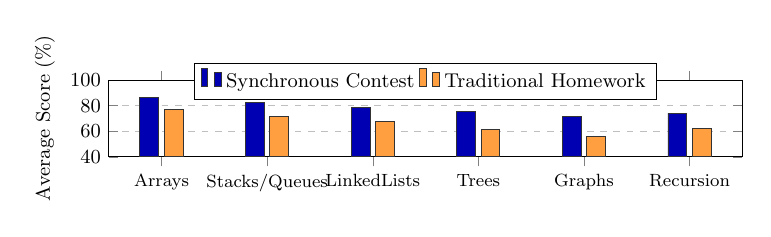
\begin{tikzpicture}[scale=0.80]
\begin{axis}[
    ybar=2.5pt,
    bar width=8.5pt,
    width=0.96\linewidth,
    height=2.8cm,
    ymin=40, ymax=100,
    ylabel={Average Score (\%)},
    symbolic x coords={Arrays, Stacks/Queues, LinkedLists, Trees, Graphs, Recursion},
    xtick=data,
    x tick label style={font=\footnotesize},
    ymajorgrids=true,
    grid style=dashed,
    legend style={at={(0.5,1.22)}, anchor=north, legend columns=2, font=\small},
    font=\small
]
\addplot[fill=blue!70!black, draw=black!80] coordinates {
    (Arrays, 86.2) (Stacks/Queues, 82.5) (LinkedLists, 78.4) (Trees, 75.6) (Graphs, 71.8) (Recursion, 74.2)
};
\addplot[fill=orange!75!white, draw=black!80] coordinates {
    (Arrays, 76.8) (Stacks/Queues, 71.2) (LinkedLists, 67.5) (Trees, 61.4) (Graphs, 55.6) (Recursion, 62.0)
};
\legend{Synchronous Contest, Traditional Homework}
\end{axis}
\end{tikzpicture}
\caption{Topic-wise practical exam scores under both instructional formats.}
\label{fig:topic_scores}
\end{figure}

Figure~\ref{fig:topic_scores} breaks down exam scores by data structure topic. Performance was higher under contest mode across all topics, with the most pronounced improvements in complex subjects: \textbf{Trees} ($+14.2\%$) and \textbf{Graphs} ($+16.2\%$). In homework mode, students struggled with pointer updates and recursion edge cases when working alone, whereas the contest environment motivated them to work through these cases during lab hours with faculty assistance.

\subsection{Problem-Solving Habits and Debugging Discipline (RQ2)}
Table~\ref{tab:debugging_metrics} presents key submission and debugging metrics extracted from platform system logs across the semester.

\begin{table}[!htbp]
\centering
\small
\caption{Problem-Solving and Submission Metrics Across Modalities}
\label{tab:debugging_metrics}
\begin{tabularx}{\linewidth}{|l|X|c|c|}
\hline
\textbf{Metric} & \textbf{Operational Definition} & \textbf{Contest Mode} & \textbf{Homework Mode} \\
\hline
Submissions per Problem & Average submission attempts until Accepted & $\mathbf{3.2 \pm 1.2}$ & $5.7 \pm 2.6$ \\
\hline
Sample Runs per Problem & In-browser sample checks before formal Submit & $\mathbf{4.8 \pm 1.8}$ & $2.1 \pm 1.4$ \\
\hline
Compilation Errors & Percentage of all formal submission events & $\mathbf{5.2\%}$ & $12.4\%$ \\
\hline
First-Attempt Accepted & Problems solved on the first submission attempt & $\mathbf{38.5\%}$ & $22.1\%$ \\
\hline
Average Time (Easy) & Minutes taken to solve an Easy problem & $14.2 \pm 4.5$ & $21.5 \pm 8.2$ \\
\hline
Average Time (Medium) & Minutes taken to solve a Medium problem & $31.4 \pm 9.8$ & $45.8 \pm 15.3$ \\
\hline
\end{tabularx}
\end{table}

A notable result is the reduction in submission attempts: students averaged $3.2$ formal submissions per solved problem in contest rooms, compared to $5.7$ in homework mode. In homework mode, students often submitted slightly edited code repeatedly to see what the server would output. In contest sessions, students made more frequent use of the ``Run Code'' button ($4.8$ runs vs. $2.1$ runs per task), testing sample inputs and checking their logic on paper before submitting. Compilation errors dropped from $12.4\%$ to $5.2\%$, reflecting greater care with syntax.

\begin{figure}[!htbp]
\centering
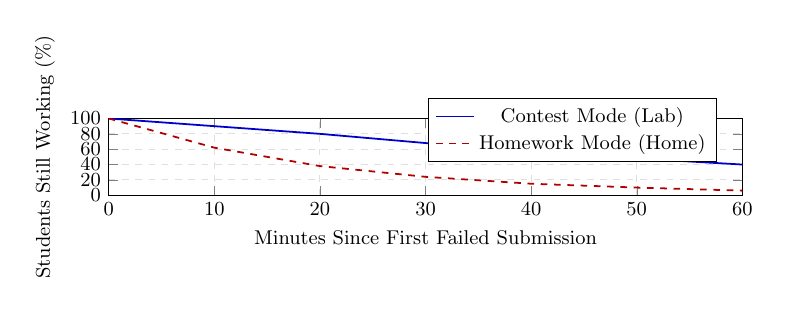
\begin{tikzpicture}[scale=0.80]
\begin{axis}[
    width=0.96\linewidth,
    height=2.8cm,
    xmin=0, xmax=60,
    ymin=0, ymax=100,
    xlabel={Minutes Since First Failed Submission},
    ylabel={Students Still Working (\%)},
    grid=both,
    grid style={dashed, gray!25},
    legend style={at={(0.96,0.85)}, anchor=east, font=\small},
    font=\small
]
\addplot[thick, blue!80!black] coordinates {
    (0, 100) (10, 90) (20, 80) (30, 68) (40, 56) (50, 48) (60, 40)
};
\addplot[thick, red!70!black, dashed] coordinates {
    (0, 100) (10, 62) (20, 38) (30, 24) (40, 15) (50, 10) (60, 6)
};
\legend{Contest Mode (Lab), Homework Mode (Home)}
\end{axis}
\end{tikzpicture}
\caption{Student persistence curve after an initial failed submission.}
\label{fig:persistence}
\end{figure}

Figure~\ref{fig:persistence} shows student persistence after receiving an initial incorrect verdict (Wrong Answer or Time Limit Exceeded). In contest mode, $40\%$ of students continued working on the problem for at least 60 minutes. In homework mode, only $6\%$ persisted past 60 minutes, with most students abandoning the task until shortly before the deadline.

\subsection{Laboratory Completion and Engagement (RQ3)}
In traditional practicals at RCPIT, only $61.2\%$ of assigned problems were finished during the two-hour lab slot. The remaining problems became homework, where $64.8\%$ of submissions were made in the final 12 hours before Sunday midnight.

Under the synchronous contest format, students completed an average of $88.5\%$ of assigned problems within the scheduled lab period. Knowing they had a 90-minute active window, students started promptly and stayed focused. Instructors were also able to help students at the moment they encountered problems, rather than answering urgent queries on Sunday evening.

% =========================================================================
\section{Student Perceptions and Fairness (RQ4)}
\label{sec:perceptions}
% =========================================================================

\subsection{Survey Feedback}
At the end of the semester, students completed an anonymous 5-point Likert scale survey ($1 = \text{Strongly Disagree}$, $5 = \text{Strongly Agree}$). Table~\ref{tab:survey_results} shows student responses.

\begin{table}[!htbp]
\centering
\small
\caption{Student Survey Feedback Responses ($N = 64$)}
\label{tab:survey_results}
\begin{tabularx}{\linewidth}{|X|c|c|c|}
\hline
\textbf{Survey Prompt} & \textbf{Mean} & \textbf{Std Dev} & \textbf{\% Agree / Strongly Agree} \\
\hline
1. Timed contest rooms helped me stay focused during practical hours. & 4.31 & 0.72 & $87.5\%$ (56 / 64) \\
\hline
2. I prefer contest-driven practicals over take-home programming assignments. & 4.38 & 0.69 & $84.4\%$ (54 / 64) \\
\hline
3. Seeing sample test results helped me debug without guessing. & 4.52 & 0.61 & $92.2\%$ (59 / 64) \\
\hline
4. The live room leaderboard motivated me rather than making me anxious. & 4.12 & 0.81 & $81.3\%$ (52 / 64) \\
\hline
5. The 30-minute post-contest review session helped clarify difficult concepts. & 4.45 & 0.66 & $89.1\%$ (57 / 64) \\
\hline
\end{tabularx}
\end{table}

Students responded very positively to the format. $87.5\%$ agreed that the live room helped them stay focused during practical hours, and $84.4\%$ preferred contest practicals over take-home homework. Importantly, $81.3\%$ reported low stress because grading was based on whether problems were solved correctly, not on leaderboard rank.

\subsection{Gender Balance and Inclusivity}
We evaluated whether contest rooms created disparate outcomes across gender. Female students gained an average of $+5.8$ marks out of 50, and male students gained an average of $+6.1$ marks. The difference between genders was not statistically significant ($t = 0.62$, $p = 0.54$). In qualitative feedback, female students noted that objective automated test cases made evaluation transparent, and they appreciated having dedicated time for instructor questions during the review session.

% =========================================================================
\section{Practical Lessons for Engineering Colleges}
\label{sec:lessons}
% =========================================================================

Based on our deployment of Campus Lab at RCPIT Shirpur, we outline four practical recommendations for computer science and engineering colleges:
\begin{enumerate}[leftmargin=1.5em, itemsep=1.5pt]
    \item \textbf{Separate Run Code from Submit Code:} Providing students with free execution against visible sample cases prevents trial-and-error submissions and encourages deliberate testing.
    \item \textbf{Grade Problem Completion, Not Speed:} Leaderboards create healthy in-lab engagement. However, official practical marks should depend entirely on solving problems correctly, ensuring that students of all typing and thinking speeds feel supported.
    \item \textbf{Structure the Two-Hour Lab Period:} Schedule a 10-minute concept introduction, a 75-to-80-minute contest session, and a 30-minute code review where instructors explain common errors and optimal approaches.
    \item \textbf{Deploy Locally on LAN:} Running the web platform, database, and Judge0 sandbox on an institutional server avoids internet downtime and delivers fast sub-second compile-run responses for all students.
\end{enumerate}

% =========================================================================
\section{Threats to Validity and Limitations}
\label{sec:threats}
% =========================================================================

Our study has three main limitations:
\begin{itemize}[leftmargin=1.5em, itemsep=1.5pt]
    \item \textbf{Single-Institution Scope:} The study was conducted within the AI\&ML department of one engineering college. While the student background and curriculum are representative of Indian undergraduate colleges, multi-institution studies will provide broader confirmation.
    \item \textbf{Course Subject:} The study examined Data Structures and Algorithms, where problems have well-defined inputs and expected outputs. Applying contest models to open-ended subjects (such as Web Development or Machine Learning modeling) requires different assessment mechanisms.
    \item \textbf{Instructor Presence:} Both practical batches had active instructor guidance during lab sessions. In settings with less hands-on faculty supervision, learning outcomes may vary.
\end{itemize}

% =========================================================================
\section*{Conclusion}
\addcontentsline{toc}{section}{Conclusion}
% =========================================================================
This paper presented Campus Lab, an open-source platform that transforms unstructured college computer practicals into active, timed contest rooms. In a 16-week crossover study with 64 AI\&ML students at RCPIT Shirpur, synchronous contest practicals increased lab completion from $61.2\%$ to $88.5\%$, raised practical exam marks by $5.8$ points out of 50, and reduced guess-and-check submissions from $5.7$ to $3.2$ per task. When grading is tied to problem correctness rather than leaderboard speed, contest-driven lab practicals provide an engaging, equitable, and effective learning environment for engineering students.

% =========================================================================
\section*{References}
\addcontentsline{toc}{section}{References}
% =========================================================================
\begin{enumerate}[label={[\arabic*]}, leftmargin=1.8em, itemsep=0pt, parsep=0pt]
    \item Joint Task Force on Computing Curricula, ``Computing Curricula 2020: Paradigms for Global Computing Education,'' \textit{ACM and IEEE Computer Society Joint Report}, 2020.
    \item S. S. Skiena and M. A. Revilla, \textit{Programming Challenges: The Programming Contest Training Manual}. New York, NY: Springer-Verlag, 2003.
    \item C. Douce, D. Livingstone, and J. Orwell, ``Automatic test-based assessment of programming: A review,'' \textit{ACM Journal on Educational Resources in Computing}, vol. 5, no. 3, pp. 1--13, 2005.
    \item H. Keuning, J. Jeuring, and B. Heeren, ``A systematic literature review of automated feedback generation for programming exercises,'' \textit{ACM Transactions on Computing Education}, vol. 19, no. 1, pp. 1--43, 2018.
    \item J. Spacco, D. Hovemeyer, W. Pugh, F. Emad, J. K. Hollingsworth, and N. Padua-Perez, ``Tracking student effort in computer science courses,'' in \textit{Proc. 37th SIGCSE Technical Symposium on Computer Science Education}, pp. 336--340, 2006.
    \item M. C. Jadud, ``Methods and tools for exploring novice compilation behaviour,'' in \textit{Proc. 2nd International Workshop on Computing Education Research}, pp. 73--84, 2006.
    \item J. Hamari, J. Koivisto, and H. Sarsa, ``Does gamification work? -- A literature review of empirical studies on gamification,'' in \textit{Proc. 47th Hawaii International Conference on System Sciences}, pp. 3025--3034, 2014.
    \item R. M. Ryan and E. L. Deci, ``Self-determination theory and the facilitation of intrinsic motivation, social development, and well-being,'' \textit{American Psychologist}, vol. 55, no. 1, pp. 68--78, 2000.
    \item S. Wasik, M. Celary, M. Fabrykiewicz, and A. Szymański, ``A survey on online judge systems and their role in computer science education and competitive programming,'' \textit{ACM Computing Surveys}, vol. 51, no. 1, pp. 1--36, 2018.
    \item E. Ihantola, T. Ahoniemi, V. Karavirta, and O. Seppälä, ``Review of recent systems for automatic assessment of programming assignments,'' in \textit{Proc. 10th Koli Calling International Conference on Computing Education Research}, pp. 86--93, 2010.
    \item S. H. Edwards, ``Using software testing to move students from trial-and-error to reflection-in-action,'' \textit{ACM SIGCSE Bulletin}, vol. 36, no. 1, pp. 26--30, 2004.
    \item B. A. Becker, G. Glacheva, J. Carter, et al., ``50 years of CS1 at SIGCSE: A review of empirical research (1970--2019),'' in \textit{Proc. 51st ACM Technical Symposium on Computer Science Education}, pp. 338--344, 2020.
    \item S. Combéfis, G. Beresnevičius, and V. Dagiene, ``Learning programming through games and contests: Overview, parallelisms and trends,'' \textit{Informatics in Education}, vol. 15, no. 1, pp. 1--14, 2016.
    \item M. S. Ribas, L. O. Brandao, and A. A. Brandao, ``Interactive automated assessment in programming labs: A competitive learning perspective,'' \textit{IEEE Transactions on Learning Technologies}, vol. 14, no. 4, pp. 512--524, 2021.
    \item L. E. Richter, F. Berger, and R. Wilder, ``Leaderboards in educational contexts: Friend or foe for student self-efficacy?,'' \textit{Computers \& Education}, vol. 182, p. 104468, 2022.
    \item D. Zou, H. Xie, F. L. Wang, and K. S. Cheung, ``A study on the motivational dynamics of leaderboard-based programming competitions,'' \textit{Educational Technology Research and Development}, vol. 69, pp. 2215--2239, 2021.
    \item M. Guzdial and E. Forte, ``Design process for a non-majors computing course,'' \textit{ACM SIGCSE Bulletin}, vol. 37, no. 1, pp. 361--365, 2005.
\end{enumerate}

\end{document}
